\chapter{Introduction}
\label{Chapter1}
\lhead{Chapter 1. \emph{Introduction}}

This first chapter ..\\

\section{Javascript}

In order to keep up with the evolution and continuous growth of the Internet,
web technologies have been undergoing significant upgrades. Since 2007, the
World Wide Web Consortium (W3C) has been working on a major update of the core
language of the web that renders and displays all web contents. This is known
as the 5th revision of Hyper Text Markup Language (HTML5).  However the slow
performance of JavaScript in performing dynamic operations is a serious
limiting factor to wider use. Improving the efficiency of JavaScript is an
active field of research.\\


CHANGE !!!!!!!!!!!!!!!!!!!!!!!!!!!!!!!!!!

\section{Client server communications}

This section studies the evolution of client server communication, beginning
with the page by page model until current technologies. However as an
introduction, the first part is about HTPP which is the fundation of client
server communication.

\subsection{HTTP protocol}

The HTTP protocol is a request/response protocol defined in the request for
comment (RFC) \cite{Reference1} as follows:

\begin{verbatim} 
A client sends a request to the server in the form of a request 
method, URI, and protocol version, followed by a MIME-like 
message containing requestmodifiers, client information, and 
possible body content over a connection with a server. The 
server responds with a status line, including the message's
protocol version and a success or error code, followed by a 
MIME-like message containing server information, entity meta 
information, and possible entity-body content.  
\end{verbatim}

Because HTTP was not designed for real time communication several workarounds
have been developped over the years to over come the so called page by page
model. These techniques are nicely resumed in Eliot Step master thesis
\citep{Reference2}.

\subsection{Page by page model}

Since HTTP's release in 1991, client-server communication have undergone
continuous upgrades. In the early nineties, most web pages were static. As a
consequence, the communication between client and server  were rather limited.
Typically, the client would send occasional request to the server. The server
would then answer but all communication would stop there until a new event was
triggered by the user.\\ 


\begin{figure}[H]
\centering
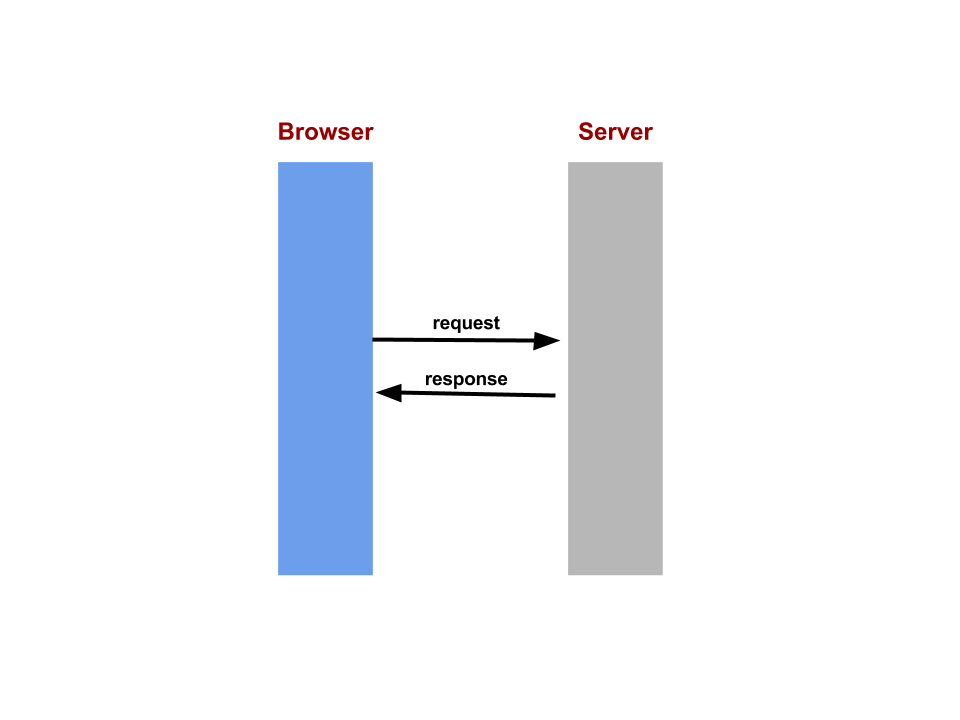
\includegraphics[width=0.9\textwidth]{./Figures/client_server_communication.png}
\caption[Client server communication]{Client server communication}
\label{fig:client_server_communication}
\end{figure}

The notion of dynamic web appeared in 2005 with the introduction of technologies
like Comet. Peter Lubbers describes it as the Headache 2.0 in his article
\texttt{A quantum leap in scalability for the web} \citep{Reference32}.\\

\subsection{Polling}

Polling was the first attempt toward real-time communication. Instead of waiting
for the client to manually ask for a page update, the browser would send regular
HTTP GET requests to the server. This technique could be efficient if the exact
interval of update on the server side was known.\\

\begin{figure}[H]
\centering
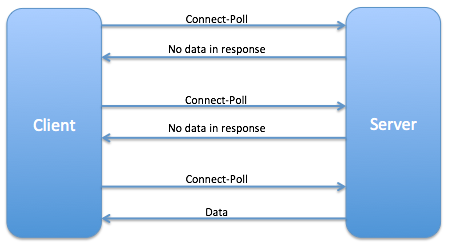
\includegraphics[width=\textwidth]{./Figures/polling.png}
\caption[Polling]{polling}
\label{fig:polling}
\end{figure}

However real time information are unpredictable and in high updates rate
situation like for example stock prices, news reports or tickets sales the
response could be stale by the time the browser renders the page
\citep{Reference32}.\\

Also in low updates rate situation even if no data is available, the server
will send an empty response. Resulting in a large amount of unnecessary
connections beeing established which over time and with the clients increase
leads to decreased overall network throughput \citep{Reference2}. \\


\subsection{Long polling}

Long polling is based on Comet technologies and is a slight step further toward
server sent events and real time communication. Comet began to be popular in web
browser around 2007, it is a family of web techniques that allows the server to
hold an HTTP request open for prolonged periods of time.\\

\begin{figure}[H]
\centering
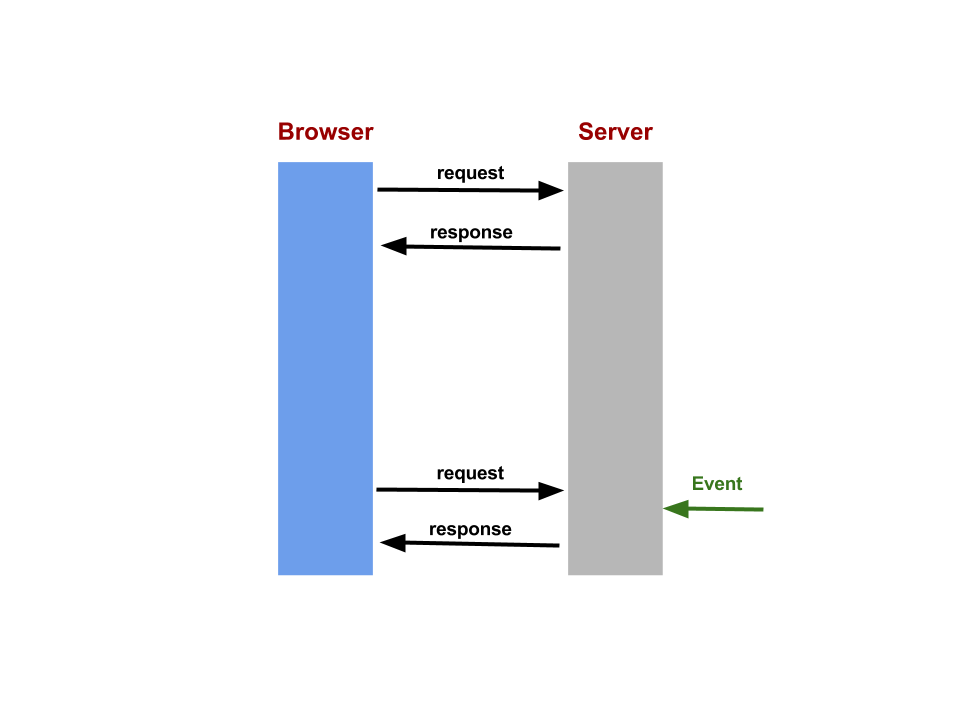
\includegraphics[width=0.9\textwidth]{./Figures/long_polling.png}
\caption[Long polling]{Long polling}
\label{fig:long_polling}
\end{figure}

Long-polling is similar to polling, except that the server keeps the HTTP
request open if data is not immediately available. The server determines how
long to keep the request open, request also known as a \texttt{hanging GET}. If
new data is received within the time interval, a response containing the data
is sent to the client and the connection is closed. If new data is not received
within the time period, the server will respond with a notification to
terminate the open request and close the connection. After the client browser
receives the response, it will create another  request to handle the next
event, therefore always keeping a new long-polling request open for new events.
This results in the server constantly responding with new data as soon as it is
made available \citep{Reference2}.\\

However, in situations with high-message volume, long- polling does not provide
increased performance benefits over regular polling. Performance could actually
be decreased if long-polling requests turn into continuous, unthrottled loops
of regular polling requests.\\


\subsection{Streaming}

Streaming is based on a persistent HTTP connection. The communication still
begins with a request from the browser, the difference is in the response. The
server never signals the browser its message is finished. This way the
connection is kept open and ready to deliver futher data \citep{Reference2}.\\

\begin{figure}[H]
\centering
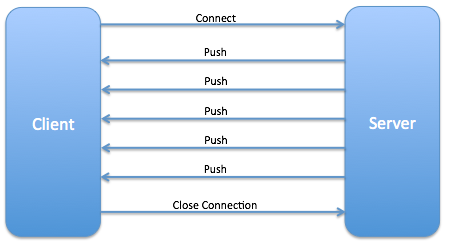
\includegraphics[width=0.9\textwidth]{./Figures/streaming.png}
\caption[Streaming]{Streaming}
\label{fig:streaming}
\end{figure}

Wouldn't it be because of proxies, streaming would be perfectly adapted for
real time communication. Because streaming is done over HTTP, proxy server may
choose to buffer server responses and thus increasing greatly the latency of
the message delivery. Therefore in case a proxy is detected most Comet-like
solution fall back to long polling \citep{Reference2}.\\

\subsection{Current technologies in browser}

At the moment, comet technologies are still the most popular way of
communication between browsers and servers. Techniques has been improved to
the point where it perfectly fakes server sent event. Comet technologies can be
seen as a wonderful hack to reach real time communication. However little can
be done to improve the latency. Comet technologies resolve around HTTP and
carry its overhead.\\

The total overhead from the HTTP request and response header is at least 871
bytes without containing any data. In comparaison, a small payload is 20 bytes.
Contempory application like on-line games can not be built on a technology
waisting ressources equivalent to 40 messages every time informations are
exchanged \citep{Reference2}. Therefore a brand new protocol has been
developed: WebSocket.\\

\section{WebSocket protocol}

The creation of the WebSocket protocol marks the begenning of the Living web.
It is often referred to as the first major upgrade in the history of web
communications. As the Web itself originally did, WebSocket enables entirely
new kinds of applications. Daily, new products are designed to stay permanently
connected to the web. Websocket is the language enabling this revolution.\\

This section is a study of the WebSocket protocol. To begin with it defines the
protocol. Secondly it studies how to establish a WebSocket connection.
Afterwards it goes on with an in depth study of WebSockets' transport layer and
frame anatomies. And to finish it provides a brief discussion of WebSockets'
interaction with proxies.

\subsection{Definition}

The official Request For Comments \citep{Reference12} (RFC) describes the
WebSocket protocol as follows:

\begin{verbatim}
The WebSocket Protocol enables two-way communication between a 
clientrunning untrusted code in a controlled environment to a 
remote host that has opted-in to communications from that code.
The security model used for this is the origin-based security 
model commonly used by web browsers. The protocol consists of an
opening handshake followed by basic message framing, layered over
TCP. The goal of this technology is to provide a mechanism for
browser-based applications that need two-way communication with
servers that does not rely on opening multiple HTTP connections.
\end{verbatim}

To iniate a WebSocket communication, first a HTTP handshake needs to be done.

\subsection{The WebSocket handshake}

The Websocket protocol was to be released in an already existing web
infrastrucure. Therefore it has been designed to be backward-compatible. Before
a Websocket communication can start, a HTTP connection must be initiated. The
browser sends an Upgrade header to the server to inform him he wants to start a
WebSocket connection. Switching from the HTTP protocol to the WebSocket
protocol is referred to as a handshake \citep{Reference12}.

\begin{verbatim}
GET ws://websocket.example.com/ HTTP/1.1
Origin: http://example.com
Connection: Upgrade
Host: websocket.example.com
Upgrade: websocket
\end{verbatim}

If the server supports the WebSocket protocol, it sends the following header in
response.

\begin{verbatim}
HTTP/1.1 101 WebSocket Protocol Handshake
Date: Wed, 5 May 2014 04:04:22 GMT
Connection: Upgrade
Upgrade: WebSocket
\end{verbatim}

After the completion of the handshake the WebSocket connection is active and
either the client or the server can send data. The data is contained in frames,
each frame is prefixed with a 4-12 bytes to ensure the message can be
reconstructed. \\ 

Once the server and the browser have agreed on begenning a WebSocket
communication. A first request is made to begin an ethernet communication
followed by a request to make an TCP / IP communication.\\

\subsection{Transport layer protocol}

The internet is based on two transport layer protocols, the User Datagram
Protocol (UDP) and the Transmission Control Protocol (TCP). Both use the
network layer service provided by the internet protocol (IP). \\

\textbf{TCP}

TCP is a reliable transmission protocol. The data is buffered bytes by bytes in
segments and transmitted according to specific timers. This flow control
ensure the consistancy of the data. TCP is said to be a stream oriented
because the data is sent in independent segments.\\

\textbf{UDP}

UDP is unreliable but fast. The protocol offers no guarenty the data will be
delivered in its integrality nor duplicated. It works on a best effort strategy
with no flow control. Each segments are received independently, it is a message
oriented protocol.\\

Websocket is build over TCP because of its realiability. Browser enabled games
are the perfect example of WebSockets' use cases. They require low latency and
have a high rate of update. To achieve low latency, the communication protocol
must make sure not to drop any packets. Otherwise, the exhange takes two times
longer.\\

As can be inferred from the 2 previous subsections, the websockets protocol
relies on a few other protocols. Namely HTTP to initialize the communication ,
ethernet, TCP/IP and finaly TLS in case a secure connections is required.  The
next subsections studies the influence this protocols have in the anatomy of
WebSockets frame.\\

\subsection{The WebSocket frame anatomy}

The study conducted by Tobias Oberstein \citep{Reference30} looks into the
overheads of websockets. As a matter of fact the overhead induced purely by
WebSockets is extremely low. As can be seen in the figure
\ref{fig:frameOverhead}, depending on the size of the payload the overhead
varies between 8 and 20 bytes.\\

\begin{figure}[H]
\centering
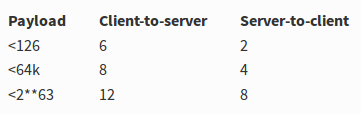
\includegraphics[width=0.6\textwidth]{./Figures/frame_overhead.png}
\caption[Frame overhead]{Frame overhead \citep{Reference30}}
\label{fig:frame_overhead}
\end{figure}

However, as pointed out in the article efficiency is lost on protocols of other layers
required for WebSocket's functionement. Figure \ref{fig:tlsOverhead} and
\ref{fig:tcpOverhead} respectively show the overhead induced by pure TCP/IP and
TLS protocols.\\

\begin{figure}[H]
\centering
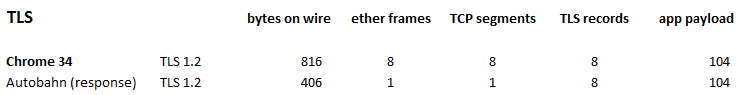
\includegraphics[width=\textwidth]{./Figures/tls_overhead.png}
\caption[TLS overhead]{TLS overhead \citep{Reference30}}
\label{fig:tls_overhead}
\end{figure}

\begin{figure}[H]
\centering
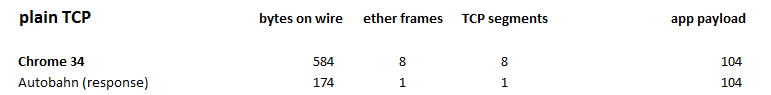
\includegraphics[width=\textwidth]{./Figures/tcp_overhead.png}
\caption[TCP overhead]{TCP overhead \citep{Reference30}}
\label{fig:tcp_overhead}
\end{figure}



In this example, the payloads \texttt{Hello world} is only thirteen bytes. In
comparaison ethernet, TCP/IP and TLS protocols each use height bytes. The
conclusion of this article is to warn programmers about the size of the
payloads to make all the protocols revolving around WebSockets don't dwarf the
overhead of the WebSocket protocol itself. In case small payloads can not be
avoided a possible solution is to serialize the messages in order to batch them
in one single WebSocket message.\\

So instead of sending the each messages using the WebSocket protocol like it is
done in figure \ref{fig:seperate_websocket}. The individual messages are put in
a queue and batched in a single Websocket message like in figure
\ref{fig:batched_websocket}.\\


\begin{figure}[H]
\centering
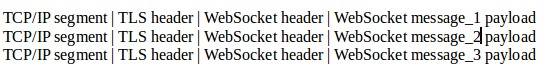
\includegraphics[width=\textwidth]{./Figures/separate_websocket.png}
\caption[Websocket messages sent individualy]{WebSocket messages sent individualy \citep{Reference30}}
\label{fig:separate_websocket}
\end{figure}

\vspace{10 mm}

\begin{figure}[H]
\centering
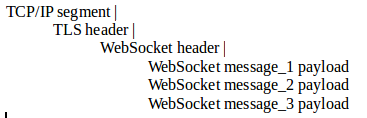
\includegraphics[width=0.7\textwidth]{./Figures/batched_websocket.png}
\caption[Batched WebSocket messages]{Batched WebSocket messages \citep{Reference30}}
\label{fig:batched_websocket}
\end{figure}

Never the less, WebSockets carry way less overhead then comet technologies do.
Another advantage of WebSocket its interaction with proxies.\\

\subsection{Proxies}

Proxy servers are set up between a private network and the Internet. They act
like an intermediary providing content caching, security and content
filtering.\\

When a Websocket server detects the presence of a proxy server, it
automatically sets up a tunnel to pass through the proxy. The tunnel is
established by issuing an HTTP CONNECT statement to the proxy server, which
requests for the proxy server to open a TCP/IP connection to a specific host
and port. Once the tunnel is set up, communication can flow unimpeded through
the proxy.\\

LINK

